%%%%%%%%%%%%%%%%%%%%%%%%%%%%%%%%%%%%%%%%%
% University/School Laboratory Report
% LaTeX Template
% Version 3.1 (25/3/14)
%
% This template has been downloaded from:
% http://www.LaTeXTemplates.com
%
% Original author:
% Linux and Unix Users Group at Virginia Tech Wiki 
% (https://vtluug.org/wiki/Example_LaTeX_chem_lab_report)
%
% License:
% CC BY-NC-SA 3.0 (http://creativecommons.org/licenses/by-nc-sa/3.0/)
%
%%%%%%%%%%%%%%%%%%%%%%%%%%%%%%%%%%%%%%%%%

%----------------------------------------------------------------------------------------
%	PACKAGES AND DOCUMENT CONFIGURATIONS
%----------------------------------------------------------------------------------------

\documentclass{article}

\usepackage{graphicx} % Required for the inclusion of images
\usepackage{amsmath} % Required for some math elements 
\usepackage{cite}
\usepackage{subcaption} %Required to group figures
\usepackage{float}

\setlength\parindent{0pt} % Removes all indentation from paragraphs

%\usepackage{times} % Uncomment to use the Times New Roman font

%----------------------------------------------------------------------------------------
%	DOCUMENT INFORMATION
%----------------------------------------------------------------------------------------

\title{Lab 2\\ Signal Generation\\ EE 445S} % Title

\author{Enoc \textsc{Balderas}} % Author name

\date{\today} % Date for the report

\begin{document}

\maketitle % Insert the title, author and date

\begin{center}
\begin{tabular}{l r}
Date Performed: & February 4, 2019 \\ % Date the experiment was performed
Partners: & Daniel Diamont \\ % Partner names
Instructor: & Professor Evans % Instructor/supervisor
\end{tabular}
\end{center}

% If you wish to include an abstract, uncomment the lines below
% \begin{abstract}
% Abstract text
% \end{abstract}

%----------------------------------------------------------------------------------------
%	SECTION 1
%----------------------------------------------------------------------------------------

\section{Introduction}

For this lab we focused on generating sinusoidal signals. 
We tested the performance and resolution of three different signal generation methods, math library function calls, difference equation, and look up table (LUT).\\

The math library function call uses an 11th order polynomial to aproximate the sinusoid.
We can use the math library function with a phase increment variable to output a sinusoid in an interrupt function.

\subsection{Difference Equation}

\begin{equation}
y[n] = sin(w_0)x[n-1] + 2cos(w_0)y[n-1] - y[n-2]
\end{equation}

The difference equation is derived from the z-transform of a causal single sided sinusoid.
Since this difference equation is derived from the transfer function of a causal single sided sinusoid, then the impulse response should be $y[n] = u[n]cos[w_0n]$.
The main advanteges of using this method are that it is not computationally intense nor does it need much memory.

\subsection{EDMA: Look Up Table}

The main benefit of having a LUT is that we can have very good resolution and not much computation.
The only drawback is that we have to store the table.
In this part of the lab we also familiarized ourselves with the EDMA hardware.
Using the EDMA has the benefit of freeing the CPU from having to handle memory transfers.

%----------------------------------------------------------------------------------------
%	SECTION 2
%----------------------------------------------------------------------------------------

\section{Methods}

\subsection{Difference Equation}

We created global variables for the desired sinusoid frequency and the initial conditions for the difference equation.
Each time the ISR is called we calculate the current value $y[n]$ and update the buffers $y[n-1]$ and $y[n-2]$.
Finally we scaled the output before writing it to the codec.

\subsection{EDMA: Look Up Table}

We calculated the $gcd(f, f_s)$ to find the number of samples needed to represent the sinosoid.
Next we used the math library calls to calculate the LUT.
 
%----------------------------------------------------------------------------------------
%	SECTION 3
%----------------------------------------------------------------------------------------

\section{Results}

\subsection{Difference Equation}

\textbf{Code:}

\begin{verbatim}
  /* variable initialization */
  if(flag == 1)
  {
    theta1 = (2*pi*6000.0/fs);
    theta2 = (2*pi*2000.0/fs);

    y1[1] = sinf(theta1);
    y2[1] = sinf(theta2);

    a1 = 2*cosf(theta1);
    a2 = 2*cosf(theta2);
    flag = 0;
  }
\end{verbatim}

\vdots

\begin{verbatim}
  /* Difference Equation */
  y1[0] = a1*y1[1] - y1[2];
  y1[2] = y1[1];
  y1[1] = y1[0];

  y2[0] = a2*y2[1] - y2[2];
  y2[2] = y2[1];
  y2[1] = y2[0];
\end{verbatim}

\begin{figure}[h]
  \begin{center}
    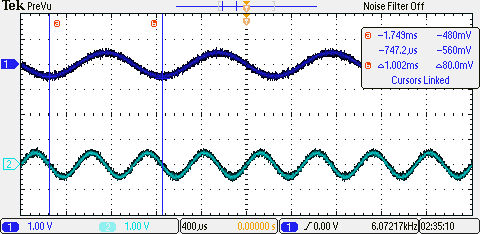
\includegraphics[width=0.65\textwidth]{img/task1.PNG}
    \caption{Blue: 1kHz Green: 2kHz.}
  \end{center}
\end{figure}

\begin{figure}[h]
  \begin{center}
    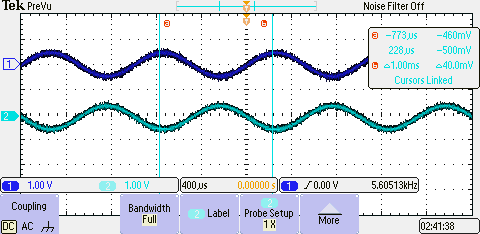
\includegraphics[width=0.65\textwidth]{img/task2.PNG}
    \caption{Blue: 1kHz Green: 7kHz.}
  \end{center}
\end{figure}

\begin{figure}[h]
  \begin{center}
    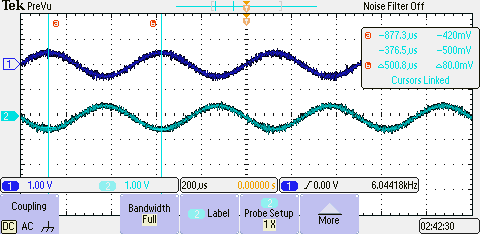
\includegraphics[width=0.65\textwidth]{img/task3.PNG}
    \caption{Blue: 2kHz Green: 6kHz.}
  \end{center}
\end{figure}

\subsection{EDMA: Look Up Table}

\textbf{Code:}

\begin{verbatim}
  place holder

  /* LUT */
  for()
  {
    buffer[][] = sin(w_0);
  }
\end{verbatim}

\begin{figure}[h]
  \begin{center}
    
\includegraphics[width=0.65\textwidth]{img/placeholder.jpg}
    \caption{Blue: 2kHz Green: 6kHz.}
  \end{center}
\end{figure}

\begin{figure}[h]
  \begin{center}
    
\includegraphics[width=0.65\textwidth]{img/placeholder.jpg}
    \caption{Blue: 2kHz Green: 6kHz.}
  \end{center}
\end{figure}

%----------------------------------------------------------------------------------------
%	SECTION 4
%----------------------------------------------------------------------------------------

\section{Discussion}

\subsection{Difference Equation}

The biggest issue we had implementing our difference equation was initializing the initial conditions.
We copied the code from the book, but we overlooked a scaling factor that seemed inconsequential.
To fix the problem we ended up changing our code a bit to make it clear what the initial conditions actually were. \\

From: \verb|y1[3] = {0 1 0}| \\
To: \verb|y1[3] = {0 sinf(w_0) 0}|

\subsection{EDMA: Look Up Table}

The LUT presented type casting challenges.
We realized that we were typecasting in the wrong order which caused us to have significant roundoff error.
We fixed our error by breaking up our statement into multiple statements.

%----------------------------------------------------------------------------------------
%	SECTION 5
%----------------------------------------------------------------------------------------

\section{Answers questions}

\subsection{Difference Equation}

\begin{enumerate}
  \begin{item}
    Explain what happened mathematically.

  \textbf{Answer:}

  \end{item}
\end{enumerate}

\subsection{EDMA: Look Up Table}

\begin{enumerate}
  \begin{item}
    Explain what happened mathematically.

  \textbf{Answer:}

  \end{item}

  \begin{item}
    Compare and contrast the three methods.

  \textbf{Answer:}

  \end{item}

  \begin{item}
    Why is scaling necessary?

  \textbf{Answer:}

  \end{item}

  \begin{item}
    How many cycles does a sin take?

  \textbf{Answer:}

  \end{item}
\end{enumerate}

%----------------------------------------------------------------------------------------
%	BIBLIOGRAPHY
%----------------------------------------------------------------------------------------

\bibliography{mybib}
\bibliographystyle{plain}

%----------------------------------------------------------------------------------------


\end{document}
